\documentclass[11pt,oneside]{book}
\usepackage[letterpaper,margin=0.72in,headheight=15pt]{geometry}
\usepackage[T1]{fontenc}
\usepackage{lmodern}
\usepackage{microtype}
\usepackage{amsmath,amssymb,mathtools}
\usepackage{array,booktabs,longtable,tabularx}
\usepackage{enumitem,multicol}
\usepackage{xcolor}
\usepackage{tikz}
\usetikzlibrary{arrows.meta,calc,decorations.pathreplacing,patterns}
\usepackage{fancyhdr}
\usepackage{titlesec}
\usepackage{hyperref}
\usepackage{bookmark}
\definecolor{navy}{HTML}{29465B}
\definecolor{steel}{HTML}{788B99}
\definecolor{pale}{HTML}{EEF3F7}
\hypersetup{colorlinks=true,linkcolor=navy,urlcolor=navy,pdftitle={Limits Drill Sheet},pdfauthor={OpenAI}}
\pagestyle{fancy}
\fancyhf{}
\fancyhead[L]{\small Limits Drill Sheet}
\fancyhead[R]{\small \thepage}
\renewcommand{\headrulewidth}{0.4pt}
\fancypagestyle{plain}{\fancyhf{}\fancyhead[L]{\small Limits Drill Sheet}\fancyhead[R]{\small \thepage}\renewcommand{\headrulewidth}{0.4pt}}
\titleformat{\chapter}[display]{\normalfont\bfseries}{\Large Topic \thechapter}{0.35em}{\Huge}
\titlespacing*{\chapter}{0pt}{-15pt}{20pt}
\setlength{\parindent}{0pt}
\setlength{\parskip}{0.55em}
\setlist{nosep}
\newenvironment{rulebox}[1]{\par\medskip\noindent{\color{navy}\bfseries #1}\par\noindent{\color{navy}\hrule}\smallskip}{\par\smallskip\noindent{\color{navy}\hrule}\par\medskip}
\newenvironment{examplebox}[1]{\par\medskip\noindent{\color{steel}\bfseries #1}\par\noindent{\color{steel}\hrule}\smallskip}{\par\smallskip\noindent{\color{steel}\hrule}\par\medskip}

\begin{document}
\frontmatter
\begin{titlepage}
\centering
\vspace*{0.8in}
{\Huge\bfseries Limits Drill Sheet\par}
\vspace{0.25in}
{\LARGE First Calculus Practice: Substitution, Algebra, Factoring, and One-Sided Limits\par}
\vspace{0.45in}
{\Large 300 progressively harder exercises: 50 per topic\par}
\vfill
\begin{rulebox}{Purpose}
This drill packet gives first-time calculus students a visual introduction to what limits mean, then repeated practice recognizing the form of a limit, choosing the correct algebraic move, and deciding when a two-sided limit exists. Each topic has fifty problems in five levels.
\end{rulebox}
\vfill
{\large Printable drill-sheet edition\par}
\end{titlepage}
\tableofcontents
\chapter*{What a Limit Is}
\addcontentsline{toc}{chapter}{What a Limit Is}
\begin{rulebox}{Main idea}
A limit describes what output value a function approaches as the input slides toward a chosen number. We are not always asking for the value at the point. We are asking what value the function is getting close to near the point.
\end{rulebox}

Imagine walking along the graph of a function. The symbol
\[
\lim_{x\to a} f(x)=L
\]
means: as your $x$-position moves closer and closer to $a$, your height on the graph moves closer and closer to $L$.

The function might actually be defined at $x=a$, or it might have a hole, a jump, or some other issue there. The limit cares about the behavior nearby. This is why a limit can exist even when $f(a)$ does not exist, and why a limit can fail to exist even when the function has values on both sides.

\section*{Sliding toward a point}
\begin{center}
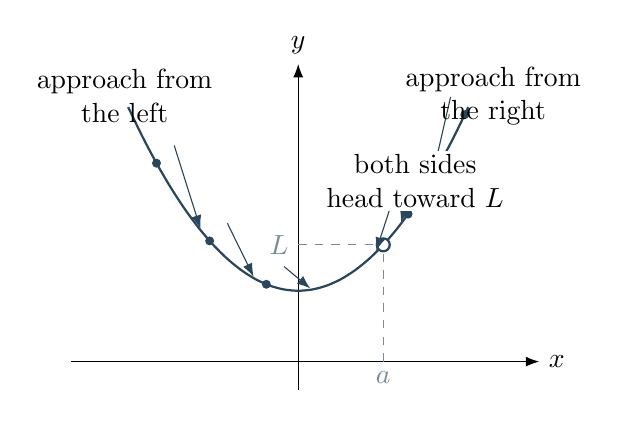
\begin{tikzpicture}[scale=0.9,>=Latex]
\draw[->] (-3.2,0) -- (3.4,0) node[right] {$x$};
\draw[->] (0,-0.4) -- (0,4.2) node[above] {$y$};
\draw[thick,navy,domain=-2.4:2.4,smooth,variable=\t] plot ({\t},{0.45*\t*\t+1});
\draw[dashed,steel] (1.2,0) node[below] {$a$} -- (1.2,1.648);
\draw[dashed,steel] (0,1.648) node[left] {$L$} -- (1.2,1.648);
\filldraw[white,draw=navy,thick] (1.2,1.648) circle (2.6pt);
\foreach \p/\lab in {-2.0/{},-1.25/{},-0.45/{}}{
  \fill[navy] (\p,{0.45*\p*\p+1}) circle (1.8pt);
  \draw[->,navy] (\p+0.25,{0.45*\p*\p+1.25}) -- (\p+0.62,{0.45*(\p+0.62)*(\p+0.62)+1.02});
}
\foreach \p in {2.35,1.9,1.55}{
  \fill[navy] (\p,{0.45*\p*\p+1}) circle (1.8pt);
  \draw[->,navy] (\p-0.2,{0.45*\p*\p+1.25}) -- (\p-0.45,{0.45*(\p-0.45)*(\p-0.45)+1.02});
}
\node[align=center] at (-2.45,3.75) {approach from\\the left};
\node[align=center] at (2.75,3.75) {approach from\\the right};
\node[align=center,fill=white,inner sep=1.5pt] at (1.65,2.55) {both sides\\head toward $L$};
\end{tikzpicture}
\end{center}

In this picture, the graph has a hole at the point above $x=a$. That hole does not automatically destroy the limit. If both sides of the graph slide toward the same height $L$, then the limit is $L$.

\section*{The value at the point is a separate question}
\begin{center}
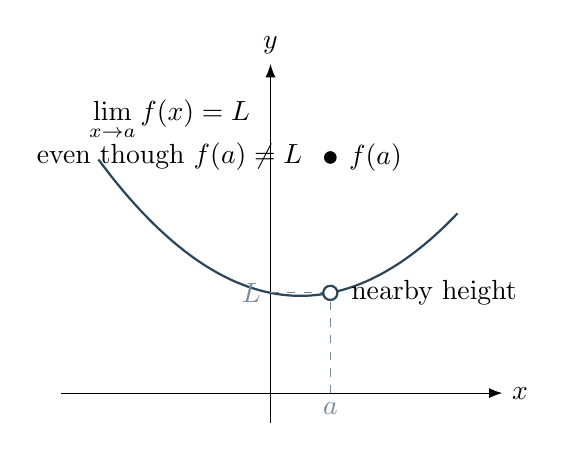
\begin{tikzpicture}[scale=0.95,>=Latex]
\draw[->] (-2.8,0) -- (3.1,0) node[right] {$x$};
\draw[->] (0,-0.4) -- (0,4.4) node[above] {$y$};
\draw[thick,navy,domain=-2.3:2.5,smooth,variable=\t] plot ({\t},{0.25*(\t-0.4)*(\t-0.4)+1.3});
\draw[dashed,steel] (0.8,0) node[below] {$a$} -- (0.8,1.34);
\draw[dashed,steel] (0,1.34) node[left] {$L$} -- (0.8,1.34);
\filldraw[white,draw=navy,thick] (0.8,1.34) circle (2.7pt);
\fill[black] (0.8,3.15) circle (2.4pt);
\node[right] at (0.92,3.15) {$f(a)$};
\node[right] at (0.95,1.34) {nearby height};
\node[align=center] at (-1.35,3.45) {$\displaystyle \lim_{x\to a}f(x)=L$\\even though $f(a)\ne L$};
\end{tikzpicture}
\end{center}

This is one of the most important habits in limits: separate the value at the point from the value approached near the point. The filled dot shows $f(a)$. The open circle shows the height the curve is approaching. The limit follows the open-circle behavior, not the filled dot.

\section*{Zooming in}
\begin{center}
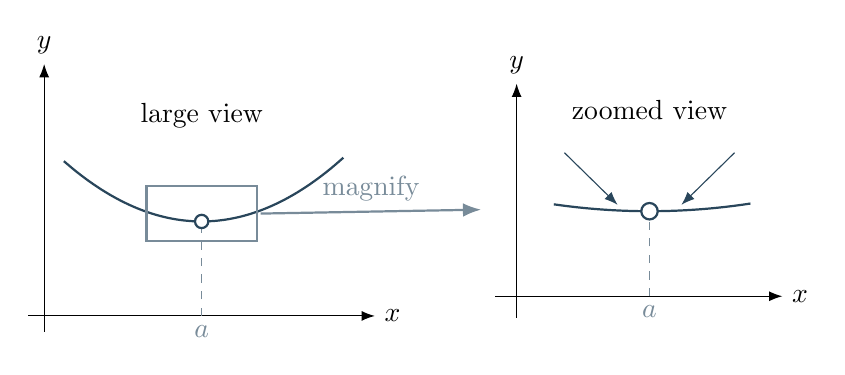
\begin{tikzpicture}[>=Latex]
\draw[->] (-0.2,0) -- (4.2,0) node[right] {$x$};
\draw[->] (0,-0.2) -- (0,3.2) node[above] {$y$};
\draw[thick,navy,domain=0.25:3.8,smooth,variable=\t] plot ({\t},{0.25*(\t-2)^2+1.2});
\draw[steel,dashed] (2,0) node[below] {$a$} -- (2,1.2);
\filldraw[white,draw=navy,thick] (2,1.2) circle (2.4pt);
\draw[steel,thick] (1.3,0.95) rectangle (2.7,1.65);
\node at (2,2.55) {large view};
\begin{scope}[xshift=6.0cm,yshift=0.25cm,scale=1.35]
  \draw[->] (-0.2,0) -- (2.5,0) node[right] {$x$};
  \draw[->] (0,-0.2) -- (0,2.0) node[above] {$y$};
  \draw[thick,navy,domain=0.35:2.2,smooth,variable=\t] plot ({\t},{0.08*(\t-1.25)^2+0.8});
  \draw[steel,dashed] (1.25,0) node[below] {$a$} -- (1.25,0.8);
  \filldraw[white,draw=navy,thick] (1.25,0.8) circle (2.2pt);
  \draw[->,navy] (0.45,1.35) -- (0.95,0.86);
  \draw[->,navy] (2.05,1.35) -- (1.55,0.86);
  \node at (1.25,1.75) {zoomed view};
\end{scope}
\draw[->,steel,thick] (2.75,1.3) -- (5.55,1.35) node[midway,above] {magnify};
\end{tikzpicture}
\end{center}

Zooming in is a good mental model. The closer $x$ gets to $a$, the more the outputs cluster near one height. In later calculus, this idea supports infinitesimal thinking: over a tiny interval, a curve can often be approximated by something simpler. Limits are the language that makes that ``tiny interval'' idea precise.

\section*{When plug-and-chug is enough}
If the expression is continuous at the target value, you may plug in the target value. This is not cheating. It is exactly what the limit laws allow. For example, polynomial expressions and rational expressions with nonzero denominators at the target value can be evaluated by substitution.

If substitution gives a normal number, stop there. The limit is that number.

\section*{When the sides matter}
Sometimes the left side and right side behave differently. Then we use one-sided limits:
\[
\lim_{x\to a^-}f(x) \qquad \text{and} \qquad \lim_{x\to a^+}f(x).
\]
The minus sign means approach from values less than $a$. The plus sign means approach from values greater than $a$.

\begin{center}
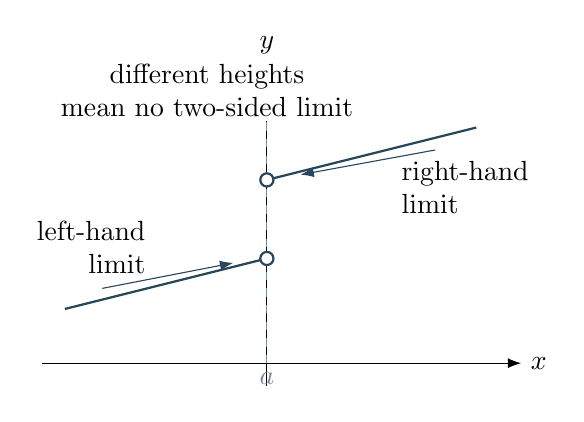
\begin{tikzpicture}[scale=0.95,>=Latex]
\draw[->] (-3,0) -- (3.4,0) node[right] {$x$};
\draw[->] (0,-0.3) -- (0,4.0) node[above] {$y$};
\draw[thick,navy,domain=-2.7:0,smooth,variable=\t] plot ({\t},{0.25*\t+1.4});
\draw[thick,navy,domain=0:2.8,smooth,variable=\t] plot ({\t},{0.25*\t+2.45});
\draw[dashed,steel] (0,0) node[below] {$a$} -- (0,3.4);
\filldraw[white,draw=navy,thick] (0,1.4) circle (2.5pt);
\filldraw[white,draw=navy,thick] (0,2.45) circle (2.5pt);
\draw[->,navy] (-2.2,1.0) -- (-0.45,1.34);
\draw[->,navy] (2.25,2.85) -- (0.45,2.52);
\node[align=right] at (-2.35,1.55) {left-hand\\limit};
\node[align=left] at (2.65,2.35) {right-hand\\limit};
\node[align=center,fill=white,inner sep=1.5pt] at (-0.8,3.65) {different heights\\mean no two-sided limit};
\end{tikzpicture}
\end{center}

Approaching from the sides is still perfectly legitimate limit work. If both one-sided limits agree, the two-sided limit exists. If they disagree, the two-sided limit does not exist.

\mainmatter

\chapter{Basic Plug-and-Chug Limits}
\begin{rulebox}{Learning target}
Evaluate limits of polynomial and simple algebraic expressions by direct substitution.
\end{rulebox}
\section*{Teaching notes}
A limit asks what value an expression approaches as $x$ gets close to a chosen number. In this first type of problem, there is no hidden obstacle: the expression is built from powers, multiplication, addition, and subtraction, so it behaves smoothly near the target value.

\subsection*{Big idea}
For polynomials and simple continuous expressions, the limit is found by replacing $x$ with the number it approaches. The arrow $x\to a$ does not mean ``$x$ equals $a$ forever.'' It means we are watching the expression as $x$ gets closer and closer to $a$.

\subsection*{Procedure}
\begin{enumerate}[leftmargin=*]
\item Identify the number that $x$ approaches.
\item Substitute that number into the expression.
\item Simplify carefully using the order of operations.
\end{enumerate}

\subsection*{Common trap}
Do not make this harder than it is. If substituting gives an ordinary real number, that number is the limit.
\begin{examplebox}{Worked example}
\textbf{Problem.} $\displaystyle \lim_{x\to 2}(3x^2-4x+1)$

\textbf{Move.} Substitute $x=2$ because polynomials are continuous.

\textbf{Result.} $3(2)^2-4(2)+1=5$.
\end{examplebox}
\section*{Drill}
\subsection*{Level I: direct recognition}
\begin{multicols}{2}
\begin{enumerate}[leftmargin=*,label=\textbf{\arabic*.},itemsep=0.65\baselineskip]
\item $\displaystyle \lim_{x \to -3} x - 4$
\item $\displaystyle \lim_{x \to -2} 2 x - 3$
\item $\displaystyle \lim_{x \to -1} 3 x - 2$
\item $\displaystyle \lim_{x \to 0} 4 x - 1$
\item $\displaystyle \lim_{x \to 1} x$
\item $\displaystyle \lim_{x \to 2} 2 x + 1$
\item $\displaystyle \lim_{x \to 3} 3 x + 2$
\item $\displaystyle \lim_{x \to 4} 4 x + 3$
\item $\displaystyle \lim_{x \to -4} x + 4$
\item $\displaystyle \lim_{x \to 5} 2 x + 5$
\end{enumerate}
\end{multicols}
\subsection*{Level II: routine variations}
\begin{multicols}{2}
\begin{enumerate}[leftmargin=*,label=\textbf{\arabic*.},itemsep=0.65\baselineskip]
\item $\displaystyle \lim_{x \to -3} x^{2} + 2 x - 3$
\item $\displaystyle \lim_{x \to -2} 2 x^{2} + x - 2$
\item $\displaystyle \lim_{x \to -1} 3 x^{2} - 1$
\item $\displaystyle \lim_{x \to 0} x^{2} - x$
\item $\displaystyle \lim_{x \to 1} 2 x^{2} - 2 x + 1$
\item $\displaystyle \lim_{x \to 2} 3 x^{2} + 2 x + 2$
\item $\displaystyle \lim_{x \to 3} x^{2} + x + 3$
\item $\displaystyle \lim_{x \to 4} 2 x^{2} - 3$
\item $\displaystyle \lim_{x \to -4} 3 x^{2} - x - 2$
\item $\displaystyle \lim_{x \to 5} x^{2} - 2 x - 1$
\end{enumerate}
\end{multicols}
\subsection*{Level III: disguised or prepared forms}
\begin{multicols}{2}
\begin{enumerate}[leftmargin=*,label=\textbf{\arabic*.},itemsep=0.65\baselineskip]
\item $\displaystyle \lim_{x \to -3} x^{2} + 7 x + 9$
\item $\displaystyle \lim_{x \to -2} x^{2} + 6 x + 3$
\item $\displaystyle \lim_{x \to -1} x^{2} + 5 x - 1$
\item $\displaystyle \lim_{x \to 0} x^{2} + 4 x - 3$
\item $\displaystyle \lim_{x \to 1} x^{2} + 3 x + 1$
\item $\displaystyle \lim_{x \to 2} x^{2} - 3 x + 3$
\item $\displaystyle \lim_{x \to 3} x^{2} - 4 x + 7$
\item $\displaystyle \lim_{x \to 4} x^{2} - 5 x + 13$
\item $\displaystyle \lim_{x \to -4} x^{2} + 12 x + 16$
\item $\displaystyle \lim_{x \to 5} x^{2} - 5 x + 24$
\end{enumerate}
\end{multicols}
\subsection*{Level IV: multi-stage execution}
\begin{multicols}{2}
\begin{enumerate}[leftmargin=*,label=\textbf{\arabic*.},itemsep=0.65\baselineskip]
\item $\displaystyle \lim_{x \to -3} x^{3} + 2 x - 7$
\item $\displaystyle \lim_{x \to -2} 2 x^{3} - x^{2} + 3 x - 7$
\item $\displaystyle \lim_{x \to -1} x^{3} - 2 x^{2} + 4 x - 7$
\item $\displaystyle \lim_{x \to 0} 2 x^{3} - 3 x^{2} + 5 x - 7$
\item $\displaystyle \lim_{x \to 1} x^{3} - 4 x^{2} + 2 x - 7$
\item $\displaystyle \lim_{x \to 2} 2 x^{3} + 3 x - 7$
\item $\displaystyle \lim_{x \to 3} x^{3} - x^{2} + 4 x - 7$
\item $\displaystyle \lim_{x \to 4} 2 x^{3} - 2 x^{2} + 5 x - 7$
\item $\displaystyle \lim_{x \to -4} x^{3} - 3 x^{2} + 2 x - 7$
\item $\displaystyle \lim_{x \to 5} 2 x^{3} - 4 x^{2} + 3 x - 7$
\end{enumerate}
\end{multicols}
\subsection*{Level V: independent mastery}
\begin{multicols}{2}
\begin{enumerate}[leftmargin=*,label=\textbf{\arabic*.},itemsep=0.65\baselineskip]
\item $\displaystyle \lim_{x \to -3} x^{3} + 5 x^{2} + 14 x + 7$
\item $\displaystyle \lim_{x \to -2} 2 x^{3} + 10 x^{2} + 28 x + 15$
\item $\displaystyle \lim_{x \to -1} 3 x^{3} + 15 x^{2} + 42 x + 23$
\item $\displaystyle \lim_{x \to 0} x^{3} + 2 x^{2} + 20 x + 7$
\item $\displaystyle \lim_{x \to 1} 2 x^{3} + 11 x^{2} + 26 x + 19$
\item $\displaystyle \lim_{x \to 2} 3 x^{3} + 16 x^{2} + 40 x + 27$
\item $\displaystyle \lim_{x \to 3} x^{3} + 3 x^{2} + 18 x + 11$
\item $\displaystyle \lim_{x \to 4} 2 x^{3} + 8 x^{2} + 32 x + 19$
\item $\displaystyle \lim_{x \to -4} 3 x^{3} + 17 x^{2} + 38 x + 31$
\item $\displaystyle \lim_{x \to 5} x^{3} + 4 x^{2} + 16 x + 15$
\end{enumerate}
\end{multicols}

\chapter{Rational Expressions by Direct Substitution}
\begin{rulebox}{Learning target}
Evaluate rational limits when the denominator is not zero at the target value.
\end{rulebox}
\section*{Teaching notes}
A rational expression is a fraction made from algebraic expressions. The main question is whether the denominator becomes zero at the target value. If the denominator does not become zero, the fraction is well-behaved there.

\subsection*{Big idea}
Direct substitution works for rational expressions whenever the denominator is not $0$. The denominator check comes first because division by zero is not allowed.

\subsection*{Procedure}
\begin{enumerate}[leftmargin=*]
\item Substitute the target value into the denominator.
\item If the denominator is not $0$, substitute into the whole fraction.
\item Simplify the numerator and denominator separately before reducing.
\end{enumerate}

\subsection*{Common trap}
Do not cancel anything unless there is a reason to factor. When direct substitution works, just substitute and simplify.
\begin{examplebox}{Worked example}
\textbf{Problem.} $\displaystyle \lim_{x\to -1}\frac{x^2+3x+5}{x+4}$

\textbf{Move.} Substitute because the denominator becomes $3$, not $0$.

\textbf{Result.} $\frac{1-3+5}{3}=1$.
\end{examplebox}
\section*{Drill}
\subsection*{Level I: direct recognition}
\begin{multicols}{2}
\begin{enumerate}[leftmargin=*,label=\textbf{\arabic*.},itemsep=0.65\baselineskip]
\item $\displaystyle \lim_{x \to -3} \frac{x - 3}{x + 10}$
\item $\displaystyle \lim_{x \to -2} \frac{2 x - 2}{x + 11}$
\item $\displaystyle \lim_{x \to -1} \frac{3 x - 1}{x + 12}$
\item $\displaystyle \lim_{x \to 0} \frac{4 x}{x + 13}$
\item $\displaystyle \lim_{x \to 1} \frac{x + 1}{x + 14}$
\item $\displaystyle \lim_{x \to 2} \frac{2 x + 2}{x + 15}$
\item $\displaystyle \lim_{x \to 3} \frac{3 x + 3}{x + 16}$
\item $\displaystyle \lim_{x \to 4} \frac{4 x + 4}{x + 17}$
\item $\displaystyle \lim_{x \to -4} \frac{x + 5}{x + 18}$
\item $\displaystyle \lim_{x \to 5} \frac{2 x + 6}{x + 19}$
\end{enumerate}
\end{multicols}
\subsection*{Level II: routine variations}
\begin{multicols}{2}
\begin{enumerate}[leftmargin=*,label=\textbf{\arabic*.},itemsep=0.65\baselineskip]
\item $\displaystyle \lim_{x \to -3} \frac{x^{2} - 2 x + 3}{x - 1}$
\item $\displaystyle \lim_{x \to -2} \frac{2 x^{2} - x + 3}{x - 3}$
\item $\displaystyle \lim_{x \to -1} \frac{3 x^{2} + 3}{x - 5}$
\item $\displaystyle \lim_{x \to 0} \frac{x^{2} + x + 3}{x - 7}$
\item $\displaystyle \lim_{x \to 1} \frac{2 x^{2} + 2 x + 3}{x - 9}$
\item $\displaystyle \lim_{x \to 2} \frac{3 x^{2} - 2 x + 3}{x - 11}$
\item $\displaystyle \lim_{x \to 3} \frac{x^{2} - x + 3}{x - 13}$
\item $\displaystyle \lim_{x \to 4} \frac{2 x^{2} + 3}{x - 15}$
\item $\displaystyle \lim_{x \to -4} \frac{3 x^{2} + x + 3}{x - 8}$
\item $\displaystyle \lim_{x \to 5} \frac{x^{2} + 2 x + 3}{x - 18}$
\end{enumerate}
\end{multicols}
\subsection*{Level III: disguised or prepared forms}
\begin{multicols}{2}
\begin{enumerate}[leftmargin=*,label=\textbf{\arabic*.},itemsep=0.65\baselineskip]
\item $\displaystyle \lim_{x \to -3} \frac{x^{2} + 3 x + 2}{x^{2} + x - 56}$
\item $\displaystyle \lim_{x \to -2} \frac{x^{2} + 3 x + 2}{x^{2} + x - 72}$
\item $\displaystyle \lim_{x \to -1} \frac{x^{2} + 3 x}{x^{2} + x - 90}$
\item $\displaystyle \lim_{x \to 0} \frac{x^{2} + 6 x + 8}{x^{2} + x - 110}$
\item $\displaystyle \lim_{x \to 1} \frac{x^{2} + 2 x + 1}{x^{2} + 5 x - 84}$
\item $\displaystyle \lim_{x \to 2} \frac{x^{2} + 2 x}{x^{2} - 64}$
\item $\displaystyle \lim_{x \to 3} \frac{x^{2} + 5 x + 6}{x^{2} - 81}$
\item $\displaystyle \lim_{x \to 4} \frac{x^{2} + 5 x + 4}{x^{2} - 100}$
\item $\displaystyle \lim_{x \to -4} \frac{x^{2} + x}{x^{2} + 4 x - 77}$
\item $\displaystyle \lim_{x \to 5} \frac{x^{2} + 4 x + 4}{x^{2} + 4 x - 96}$
\end{enumerate}
\end{multicols}
\subsection*{Level IV: multi-stage execution}
\begin{multicols}{2}
\begin{enumerate}[leftmargin=*,label=\textbf{\arabic*.},itemsep=0.65\baselineskip]
\item $\displaystyle \lim_{x \to -3} \frac{\frac{x + 1}{x + 8}}{\frac{x - 2}{x + 11}}$
\item $\displaystyle \lim_{x \to -2} \frac{\frac{2 x + 1}{x + 9}}{\frac{x - 2}{x + 12}}$
\item $\displaystyle \lim_{x \to -1} \frac{\frac{3 x + 1}{x + 10}}{\frac{x - 2}{x + 13}}$
\item $\displaystyle \lim_{x \to 0} \frac{\frac{x + 1}{x + 11}}{\frac{x - 2}{x + 14}}$
\item $\displaystyle \lim_{x \to 1} \frac{\frac{2 x + 1}{x + 12}}{\frac{x - 2}{x + 15}}$
\item $\displaystyle \lim_{x \to 2} \frac{\frac{3 x + 1}{x + 13}}{\frac{x - 2}{x + 16}}$
\item $\displaystyle \lim_{x \to 3} \frac{\frac{x + 1}{x + 14}}{\frac{x - 2}{x + 11}}$
\item $\displaystyle \lim_{x \to 4} \frac{\frac{2 x + 1}{x + 15}}{\frac{x - 2}{x + 12}}$
\item $\displaystyle \lim_{x \to -4} \frac{\frac{3 x + 1}{x + 16}}{\frac{x - 2}{x + 13}}$
\item $\displaystyle \lim_{x \to 5} \frac{\frac{x + 1}{x + 17}}{\frac{x - 2}{x + 14}}$
\end{enumerate}
\end{multicols}
\subsection*{Level V: independent mastery}
\begin{multicols}{2}
\begin{enumerate}[leftmargin=*,label=\textbf{\arabic*.},itemsep=0.65\baselineskip]
\item $\displaystyle \lim_{x \to -3} \frac{x^{3} - 2 x - 5}{x^{2} + 8 x + 30}$
\item $\displaystyle \lim_{x \to -2} \frac{2 x^{3} - 2 x - 4}{x^{2} + 9 x + 31}$
\item $\displaystyle \lim_{x \to -1} \frac{3 x^{3} - 2 x - 3}{x^{2} + 10 x + 32}$
\item $\displaystyle \lim_{x \to 0} \frac{x^{3} - 2 x - 2}{x^{2} + 11 x + 33}$
\item $\displaystyle \lim_{x \to 1} \frac{2 x^{3} - 2 x - 1}{x^{2} + 8 x + 34}$
\item $\displaystyle \lim_{x \to 2} \frac{3 x^{3} - 2 x}{x^{2} + 9 x + 35}$
\item $\displaystyle \lim_{x \to 3} \frac{x^{3} - 2 x + 1}{x^{2} + 10 x + 36}$
\item $\displaystyle \lim_{x \to 4} \frac{2 x^{3} - 2 x + 2}{x^{2} + 11 x + 37}$
\item $\displaystyle \lim_{x \to -4} \frac{3 x^{3} - 2 x + 3}{x^{2} + 8 x + 38}$
\item $\displaystyle \lim_{x \to 5} \frac{x^{3} - 2 x + 4}{x^{2} + 9 x + 39}$
\end{enumerate}
\end{multicols}

\chapter{Factoring and Cancellation Limits}
\begin{rulebox}{Learning target}
Handle $0/0$ rational limits by factoring completely, cancelling common factors, and then substituting.
\end{rulebox}
\section*{Teaching notes}
Sometimes direct substitution gives $\frac{0}{0}$. This does not mean the limit is $0$, and it does not mean the limit is undefined. It means the expression needs more algebra before the limit can be evaluated.

\subsection*{Big idea}
The form $\frac{0}{0}$ often signals a removable factor. Factor the numerator and denominator, cancel any common factor, and then evaluate the simpler expression. The cancellation does not say the original expression was defined at the target value; it says the nearby behavior can be represented by a simpler expression.

\subsection*{Procedure}
\begin{enumerate}[leftmargin=*]
\item Substitute first to see whether you get $\frac{0}{0}$.
\item Factor the numerator and denominator completely.
\item Cancel only entire common factors.
\item Substitute the target value into the simplified expression.
\end{enumerate}

\subsection*{Common trap}
Never cancel terms separated by addition or subtraction. For example, in $\frac{x+3}{x}$, the $x$ in the numerator is not a factor by itself.
\begin{examplebox}{Worked example}
\textbf{Problem.} $\displaystyle \lim_{x\to 3}\frac{x^2-9}{x-3}$

\textbf{Move.} Factor $x^2-9=(x-3)(x+3)$, cancel the common factor, then substitute.

\textbf{Result.} $6$.
\end{examplebox}
\section*{Drill}
\subsection*{Level I: direct recognition}
\begin{multicols}{2}
\begin{enumerate}[leftmargin=*,label=\textbf{\arabic*.},itemsep=0.65\baselineskip]
\item $\displaystyle \lim_{x \to 3} \frac{x^{2} - 9}{x - 3}$
\item $\displaystyle \lim_{x \to 4} \frac{x^{2} - 16}{x - 4}$
\item $\displaystyle \lim_{x \to -5} \frac{x^{2} - 25}{x + 5}$
\item $\displaystyle \lim_{x \to -2} \frac{x^{2} + 5 x + 6}{x + 2}$
\item $\displaystyle \lim_{x \to 4} \frac{x^{2} - x - 12}{x - 4}$
\item $\displaystyle \lim_{x \to -3} \frac{2 x^{2} + 7 x + 3}{x + 3}$
\item $\displaystyle \lim_{x \to 4} \frac{3 x^{2} - 11 x - 4}{x - 4}$
\item $\displaystyle \lim_{x \to 2} \frac{x^{3} - 8}{x - 2}$
\item $\displaystyle \lim_{x \to -3} \frac{x^{3} + 27}{x + 3}$
\item $\displaystyle \lim_{x \to 2} \frac{x^{4} - 16}{x - 2}$
\end{enumerate}
\end{multicols}
\subsection*{Level II: routine variations}
\begin{multicols}{2}
\begin{enumerate}[leftmargin=*,label=\textbf{\arabic*.},itemsep=0.65\baselineskip]
\item $\displaystyle \lim_{x \to 3} \frac{x^{3} - 2 x^{2} - 9 x + 18}{x^{2} + 4 x - 21}$
\item $\displaystyle \lim_{x \to 4} \frac{2 x^{3} - x^{2} - 32 x + 16}{x^{2} + 4 x - 32}$
\item $\displaystyle \lim_{x \to -5} \frac{3 x^{3} - 75 x}{x^{2} + 14 x + 45}$
\item $\displaystyle \lim_{x \to -2} \frac{x^{3} + 6 x^{2} + 11 x + 6}{x^{2} + 12 x + 20}$
\item $\displaystyle \lim_{x \to 4} \frac{2 x^{3} - 26 x - 24}{x^{2} + 3 x - 28}$
\item $\displaystyle \lim_{x \to -3} \frac{6 x^{3} + 27 x^{2} + 30 x + 9}{x^{2} + 11 x + 24}$
\item $\displaystyle \lim_{x \to 4} \frac{3 x^{3} + x^{2} - 48 x - 16}{x^{2} + 5 x - 36}$
\item $\displaystyle \lim_{x \to 2} \frac{2 x^{4} + 5 x^{3} - 16 x - 40}{x^{2} + 8 x - 20}$
\item $\displaystyle \lim_{x \to -3} \frac{3 x^{4} + 6 x^{3} + 81 x + 162}{x^{2} + 10 x + 21}$
\item $\displaystyle \lim_{x \to 2} \frac{x^{5} + 7 x^{4} - 16 x - 112}{x^{2} + 6 x - 16}$
\end{enumerate}
\end{multicols}
\subsection*{Level III: disguised or prepared forms}
\begin{multicols}{2}
\begin{enumerate}[leftmargin=*,label=\textbf{\arabic*.},itemsep=0.65\baselineskip]
\item $\displaystyle \lim_{x \to 3} \frac{x^{3} - 2 x^{2} - 6 x + 9}{x^{3} + 6 x^{2} - 9 x - 54}$
\item $\displaystyle \lim_{x \to 4} \frac{2 x^{3} - 7 x^{2} - 7 x + 12}{x^{3} + 5 x^{2} - 16 x - 80}$
\item $\displaystyle \lim_{x \to -5} \frac{3 x^{3} + 16 x^{2} + 2 x - 15}{x^{3} + 4 x^{2} - 25 x - 100}$
\item $\displaystyle \lim_{x \to -2} \frac{4 x^{3} + 9 x^{2} - x - 6}{x^{3} + 8 x^{2} + 21 x + 18}$
\item $\displaystyle \lim_{x \to 4} \frac{x^{3} - 3 x^{2} - 7 x + 12}{x^{3} + x^{2} - 14 x - 24}$
\item $\displaystyle \lim_{x \to -3} \frac{2 x^{3} + 7 x^{2} - 9}{2 x^{3} + 19 x^{2} + 45 x + 18}$
\item $\displaystyle \lim_{x \to 4} \frac{3 x^{3} - 11 x^{2} - 7 x + 12}{3 x^{3} + 4 x^{2} - 59 x - 20}$
\item $\displaystyle \lim_{x \to 2} \frac{4 x^{3} - 7 x^{2} - 5 x + 6}{x^{4} + 4 x^{3} - 8 x - 32}$
\item $\displaystyle \lim_{x \to -3} \frac{x^{3} + 4 x^{2} - 9}{x^{4} + 3 x^{3} + 27 x + 81}$
\item $\displaystyle \lim_{x \to 2} \frac{2 x^{3} - 3 x^{2} - 5 x + 6}{x^{5} + 2 x^{4} - 16 x - 32}$
\end{enumerate}
\end{multicols}
\subsection*{Level IV: multi-stage execution}
\begin{multicols}{2}
\begin{enumerate}[leftmargin=*,label=\textbf{\arabic*.},itemsep=0.65\baselineskip]
\item $\displaystyle \lim_{x \to 3} \frac{x^{3} + x^{2} - 9 x - 9}{x^{3} - x^{2} - 5 x - 3}$
\item $\displaystyle \lim_{x \to 4} \frac{x^{3} + 2 x^{2} - 16 x - 32}{x^{3} - x^{2} - 11 x - 4}$
\item $\displaystyle \lim_{x \to -5} \frac{x^{3} + 3 x^{2} - 25 x - 75}{x^{3} + 9 x^{2} + 21 x + 5}$
\item $\displaystyle \lim_{x \to -2} \frac{x^{3} + 9 x^{2} + 26 x + 24}{x^{3} + 7 x^{2} + 11 x + 2}$
\item $\displaystyle \lim_{x \to 4} \frac{x^{3} + 4 x^{2} - 17 x - 60}{x^{3} - 2 x^{2} - 7 x - 4}$
\item $\displaystyle \lim_{x \to -3} \frac{2 x^{3} + 9 x^{2} + 10 x + 3}{x^{3} + 6 x^{2} + 10 x + 3}$
\item $\displaystyle \lim_{x \to 4} \frac{3 x^{3} - 5 x^{2} - 26 x - 8}{x^{3} - 15 x - 4}$
\item $\displaystyle \lim_{x \to 2} \frac{x^{4} + 3 x^{3} - 8 x - 24}{x^{3} + 3 x^{2} - 9 x - 2}$
\item $\displaystyle \lim_{x \to -3} \frac{x^{4} + 4 x^{3} + 27 x + 108}{x^{3} + 5 x^{2} + 7 x + 3}$
\item $\displaystyle \lim_{x \to 2} \frac{x^{5} + 5 x^{4} - 16 x - 80}{x^{3} + x^{2} - 5 x - 2}$
\end{enumerate}
\end{multicols}
\subsection*{Level V: independent mastery}
\begin{multicols}{2}
\begin{enumerate}[leftmargin=*,label=\textbf{\arabic*.},itemsep=0.65\baselineskip]
\item $\displaystyle \lim_{x \to 3} \frac{x^{3} - 2 x^{2} - 5 x + 6}{x^{3} + 5 x^{2} - 9 x - 45}$
\item $\displaystyle \lim_{x \to 4} \frac{x^{3} - 3 x^{2} - 10 x + 24}{x^{3} + 6 x^{2} - 16 x - 96}$
\item $\displaystyle \lim_{x \to -5} \frac{x^{3} + 6 x^{2} - 7 x - 60}{x^{3} + 7 x^{2} - 25 x - 175}$
\item $\displaystyle \lim_{x \to -2} \frac{x^{3} + 6 x^{2} + 3 x - 10}{x^{3} + 13 x^{2} + 46 x + 48}$
\item $\displaystyle \lim_{x \to 4} \frac{x^{3} - 4 x^{2} - 4 x + 16}{x^{3} + 8 x^{2} - 21 x - 108}$
\item $\displaystyle \lim_{x \to -3} \frac{x^{3} + 3 x^{2} - 9 x - 27}{2 x^{3} + 27 x^{2} + 73 x + 30}$
\item $\displaystyle \lim_{x \to 4} \frac{x^{3} - x^{2} - 16 x + 16}{3 x^{3} + 4 x^{2} - 59 x - 20}$
\item $\displaystyle \lim_{x \to 2} \frac{x^{3} + x^{2} - 16 x + 20}{x^{4} + 6 x^{3} - 8 x - 48}$
\item $\displaystyle \lim_{x \to -3} \frac{x^{3} + 2 x^{2} - 9 x - 18}{x^{4} + 7 x^{3} + 27 x + 189}$
\item $\displaystyle \lim_{x \to 2} \frac{x^{3} - 7 x + 6}{x^{5} + 8 x^{4} - 16 x - 128}$
\end{enumerate}
\end{multicols}

\chapter{Left and Right Limits}
\begin{rulebox}{Learning target}
Evaluate left-hand and right-hand limits of piecewise functions by using the rule on the correct side of the target.
\end{rulebox}
\section*{Teaching notes}
A one-sided limit looks at the function from only one direction. The symbol $x\to a^-$ means $x$ approaches $a$ from the left, using values less than $a$. The symbol $x\to a^+$ means $x$ approaches $a$ from the right, using values greater than $a$.

\subsection*{Big idea}
For a piecewise function, the rule you use depends on the side you are approaching from. A left-hand limit uses the formula attached to $x<a$. A right-hand limit uses the formula attached to $x>a$.

\subsection*{Procedure}
\begin{enumerate}[leftmargin=*]
\item Identify the target value.
\item For $x\to a^-$, use the piece of the function for inputs less than $a$.
\item For $x\to a^+$, use the piece of the function for inputs greater than $a$.
\item Substitute $a$ into the correct side's rule.
\end{enumerate}

\subsection*{Common trap}
The value of $f(a)$, if it is even listed, does not control the one-sided limit. Limits care about nearby behavior.
\begin{examplebox}{Worked example}
\textbf{Problem.} If $f(x)=\begin{cases}x+1,&x<2\\3x,&x>2\end{cases}$, find both one-sided limits at $x=2$.

\textbf{Result.} $\lim_{x\to2^-}f(x)=3$ and $\lim_{x\to2^+}f(x)=6$.
\end{examplebox}
\section*{Drill}
\subsection*{Level I: direct recognition}
\begin{multicols}{2}
\begin{enumerate}[leftmargin=*,label=\textbf{\arabic*.},itemsep=0.65\baselineskip]
\item $f(x)=\begin{cases} x, & x<-3\\ 2 x, & x>-3 \end{cases}$; find $\lim_{x\to -3^-}f(x)$ and $\lim_{x\to -3^+}f(x)$
\item $f(x)=\begin{cases} x + 1, & x<-2\\ 2 x - 1, & x>-2 \end{cases}$; find $\lim_{x\to -2^-}f(x)$ and $\lim_{x\to -2^+}f(x)$
\item $f(x)=\begin{cases} x + 2, & x<-1\\ 2 x - 2, & x>-1 \end{cases}$; find $\lim_{x\to -1^-}f(x)$ and $\lim_{x\to -1^+}f(x)$
\item $f(x)=\begin{cases} x + 3, & x<0\\ 2 x - 3, & x>0 \end{cases}$; find $\lim_{x\to 0^-}f(x)$ and $\lim_{x\to 0^+}f(x)$
\item $f(x)=\begin{cases} x + 4, & x<1\\ 2 x - 4, & x>1 \end{cases}$; find $\lim_{x\to 1^-}f(x)$ and $\lim_{x\to 1^+}f(x)$
\item $f(x)=\begin{cases} x + 5, & x<2\\ 2 x - 5, & x>2 \end{cases}$; find $\lim_{x\to 2^-}f(x)$ and $\lim_{x\to 2^+}f(x)$
\item $f(x)=\begin{cases} x + 6, & x<3\\ 2 x - 6, & x>3 \end{cases}$; find $\lim_{x\to 3^-}f(x)$ and $\lim_{x\to 3^+}f(x)$
\item $f(x)=\begin{cases} x + 7, & x<4\\ 2 x - 7, & x>4 \end{cases}$; find $\lim_{x\to 4^-}f(x)$ and $\lim_{x\to 4^+}f(x)$
\item $f(x)=\begin{cases} x + 8, & x<-4\\ 2 x - 8, & x>-4 \end{cases}$; find $\lim_{x\to -4^-}f(x)$ and $\lim_{x\to -4^+}f(x)$
\item $f(x)=\begin{cases} x + 9, & x<5\\ 2 x - 9, & x>5 \end{cases}$; find $\lim_{x\to 5^-}f(x)$ and $\lim_{x\to 5^+}f(x)$
\end{enumerate}
\end{multicols}
\subsection*{Level II: routine variations}
\begin{multicols}{2}
\begin{enumerate}[leftmargin=*,label=\textbf{\arabic*.},itemsep=0.65\baselineskip]
\item $f(x)=\begin{cases} x^{2}, & x<-3\\ - x, & x>-3 \end{cases}$; find both one-sided limits at $x=-3$
\item $f(x)=\begin{cases} x^{2} + 1, & x<-2\\ 3 - x, & x>-2 \end{cases}$; find both one-sided limits at $x=-2$
\item $f(x)=\begin{cases} x^{2} + 2, & x<-1\\ 6 - x, & x>-1 \end{cases}$; find both one-sided limits at $x=-1$
\item $f(x)=\begin{cases} x^{2} + 3, & x<0\\ 9 - x, & x>0 \end{cases}$; find both one-sided limits at $x=0$
\item $f(x)=\begin{cases} x^{2} + 4, & x<1\\ 12 - x, & x>1 \end{cases}$; find both one-sided limits at $x=1$
\item $f(x)=\begin{cases} x^{2} + 5, & x<2\\ 15 - x, & x>2 \end{cases}$; find both one-sided limits at $x=2$
\item $f(x)=\begin{cases} x^{2} + 6, & x<3\\ 18 - x, & x>3 \end{cases}$; find both one-sided limits at $x=3$
\item $f(x)=\begin{cases} x^{2} + 7, & x<4\\ 21 - x, & x>4 \end{cases}$; find both one-sided limits at $x=4$
\item $f(x)=\begin{cases} x^{2} + 8, & x<-4\\ 24 - x, & x>-4 \end{cases}$; find both one-sided limits at $x=-4$
\item $f(x)=\begin{cases} x^{2} + 9, & x<5\\ 27 - x, & x>5 \end{cases}$; find both one-sided limits at $x=5$
\end{enumerate}
\end{multicols}
\subsection*{Level III: disguised or prepared forms}
\begin{multicols}{2}
\begin{enumerate}[leftmargin=*,label=\textbf{\arabic*.},itemsep=0.65\baselineskip]
\item $f(x)=\begin{cases} \frac{x^{2} - 9}{x + 3}, & x<-3\\ x + 2, & x>-3 \end{cases}$; find both one-sided limits at $x=-3$
\item $f(x)=\begin{cases} \frac{x^{2} - 4}{x + 2}, & x<-2\\ 2 x + 2, & x>-2 \end{cases}$; find both one-sided limits at $x=-2$
\item $f(x)=\begin{cases} \frac{x^{2} - 1}{x + 1}, & x<-1\\ 3 x + 2, & x>-1 \end{cases}$; find both one-sided limits at $x=-1$
\item $f(x)=\begin{cases} \frac{x^{2} + x}{x}, & x<0\\ x + 2, & x>0 \end{cases}$; find both one-sided limits at $x=0$
\item $f(x)=\begin{cases} \frac{x^{2} - 1}{x - 1}, & x<1\\ 2 x + 2, & x>1 \end{cases}$; find both one-sided limits at $x=1$
\item $f(x)=\begin{cases} \frac{x^{2} - 4}{x - 2}, & x<2\\ 3 x + 2, & x>2 \end{cases}$; find both one-sided limits at $x=2$
\item $f(x)=\begin{cases} \frac{x^{2} - 9}{x - 3}, & x<3\\ x + 2, & x>3 \end{cases}$; find both one-sided limits at $x=3$
\item $f(x)=\begin{cases} \frac{x^{2} - 16}{x - 4}, & x<4\\ 2 x + 2, & x>4 \end{cases}$; find both one-sided limits at $x=4$
\item $f(x)=\begin{cases} \frac{x^{2} - 16}{x + 4}, & x<-4\\ 3 x + 2, & x>-4 \end{cases}$; find both one-sided limits at $x=-4$
\item $f(x)=\begin{cases} \frac{x^{2} - 25}{x - 5}, & x<5\\ x + 2, & x>5 \end{cases}$; find both one-sided limits at $x=5$
\end{enumerate}
\end{multicols}
\subsection*{Level IV: multi-stage execution}
\begin{multicols}{2}
\begin{enumerate}[leftmargin=*,label=\textbf{\arabic*.},itemsep=0.65\baselineskip]
\item $f(x)=\begin{cases} x^{2} + 6 x + 9, & x<-3\\ \frac{x^{2} + 2 x + 1}{x + 9}, & x>-3 \end{cases}$; find $\lim_{x\to -3^-}f(x)$ and $\lim_{x\to -3^+}f(x)$
\item $f(x)=\begin{cases} x^{2} + 4 x + 5, & x<-2\\ \frac{x^{2} + x + 1}{x + 10}, & x>-2 \end{cases}$; find $\lim_{x\to -2^-}f(x)$ and $\lim_{x\to -2^+}f(x)$
\item $f(x)=\begin{cases} x^{2} + 2 x + 3, & x<-1\\ \frac{x^{2} + 1}{x + 11}, & x>-1 \end{cases}$; find $\lim_{x\to -1^-}f(x)$ and $\lim_{x\to -1^+}f(x)$
\item $f(x)=\begin{cases} x^{2} + 3, & x<0\\ \frac{x^{2} - x + 1}{x + 12}, & x>0 \end{cases}$; find $\lim_{x\to 0^-}f(x)$ and $\lim_{x\to 0^+}f(x)$
\item $f(x)=\begin{cases} x^{2} - 2 x + 5, & x<1\\ \frac{x^{2} + 2 x + 1}{x + 13}, & x>1 \end{cases}$; find $\lim_{x\to 1^-}f(x)$ and $\lim_{x\to 1^+}f(x)$
\item $f(x)=\begin{cases} x^{2} - 4 x + 9, & x<2\\ \frac{x^{2} + x + 1}{x + 14}, & x>2 \end{cases}$; find $\lim_{x\to 2^-}f(x)$ and $\lim_{x\to 2^+}f(x)$
\item $f(x)=\begin{cases} x^{2} - 6 x + 15, & x<3\\ \frac{x^{2} + 1}{x + 15}, & x>3 \end{cases}$; find $\lim_{x\to 3^-}f(x)$ and $\lim_{x\to 3^+}f(x)$
\item $f(x)=\begin{cases} x^{2} - 8 x + 23, & x<4\\ \frac{x^{2} - x + 1}{x + 16}, & x>4 \end{cases}$; find $\lim_{x\to 4^-}f(x)$ and $\lim_{x\to 4^+}f(x)$
\item $f(x)=\begin{cases} x^{2} + 8 x + 24, & x<-4\\ \frac{x^{2} + 2 x + 1}{x + 17}, & x>-4 \end{cases}$; find $\lim_{x\to -4^-}f(x)$ and $\lim_{x\to -4^+}f(x)$
\item $f(x)=\begin{cases} x^{2} - 10 x + 34, & x<5\\ \frac{x^{2} + x + 1}{x + 18}, & x>5 \end{cases}$; find $\lim_{x\to 5^-}f(x)$ and $\lim_{x\to 5^+}f(x)$
\end{enumerate}
\end{multicols}
\subsection*{Level V: independent mastery}
\begin{multicols}{2}
\begin{enumerate}[leftmargin=*,label=\textbf{\arabic*.},itemsep=0.65\baselineskip]
\item $f(x)=\begin{cases} \frac{x^{2} + 4 x + 3}{x + 3}, & x<-3\\ \frac{2 x^{2} + 6 x}{x + 3}, & x>-3 \end{cases}$; find both one-sided limits at $x=-3$
\item $f(x)=\begin{cases} \frac{x^{2} + 4 x + 4}{x + 2}, & x<-2\\ \frac{2 x^{2} + 3 x - 2}{x + 2}, & x>-2 \end{cases}$; find both one-sided limits at $x=-2$
\item $f(x)=\begin{cases} \frac{x^{2} + 4 x + 3}{x + 1}, & x<-1\\ \frac{2 x^{2} - 2}{x + 1}, & x>-1 \end{cases}$; find both one-sided limits at $x=-1$
\item $f(x)=\begin{cases} \frac{x^{2} + 4 x}{x}, & x<0\\ \frac{2 x^{2} - 3 x}{x}, & x>0 \end{cases}$; find both one-sided limits at $x=0$
\item $f(x)=\begin{cases} \frac{x^{2} + 4 x - 5}{x - 1}, & x<1\\ \frac{2 x^{2} - 6 x + 4}{x - 1}, & x>1 \end{cases}$; find both one-sided limits at $x=1$
\item $f(x)=\begin{cases} \frac{x^{2} + 4 x - 12}{x - 2}, & x<2\\ \frac{2 x^{2} - 9 x + 10}{x - 2}, & x>2 \end{cases}$; find both one-sided limits at $x=2$
\item $f(x)=\begin{cases} \frac{x^{2} + 4 x - 21}{x - 3}, & x<3\\ \frac{2 x^{2} - 12 x + 18}{x - 3}, & x>3 \end{cases}$; find both one-sided limits at $x=3$
\item $f(x)=\begin{cases} \frac{x^{2} + 4 x - 32}{x - 4}, & x<4\\ \frac{2 x^{2} - 15 x + 28}{x - 4}, & x>4 \end{cases}$; find both one-sided limits at $x=4$
\item $f(x)=\begin{cases} \frac{x^{2} + 13 x + 36}{x + 4}, & x<-4\\ \frac{2 x^{2} - 32}{x + 4}, & x>-4 \end{cases}$; find both one-sided limits at $x=-4$
\item $f(x)=\begin{cases} \frac{x^{2} + 5 x - 50}{x - 5}, & x<5\\ \frac{2 x^{2} - 19 x + 45}{x - 5}, & x>5 \end{cases}$; find both one-sided limits at $x=5$
\end{enumerate}
\end{multicols}

\chapter{One-Sided Limits That Disagree}
\begin{rulebox}{Learning target}
Compare one-sided limits and conclude that the two-sided limit does not exist when they disagree.
\end{rulebox}
\section*{Teaching notes}
A two-sided limit exists only when the left-hand and right-hand limits approach the same value. If the two sides approach different values, the function has a jump at that point, and the two-sided limit does not exist.

\subsection*{Big idea}
The two sides must agree. It is not enough for each one-sided limit to exist separately. They have to land on the same number.

\subsection*{Procedure}
\begin{enumerate}[leftmargin=*]
\item Find $\lim_{x\to a^-}f(x)$ using the left-hand rule.
\item Find $\lim_{x\to a^+}f(x)$ using the right-hand rule.
\item Compare the two answers.
\item If they are equal, the two-sided limit is that shared value. If they are different, write that the limit does not exist.
\end{enumerate}

\subsection*{Common trap}
Do not average the two one-sided limits or choose the side that looks simpler. Disagreement means the two-sided limit does not exist.
\begin{examplebox}{Worked example}
\textbf{Problem.} If $f(x)=\begin{cases}x,&x<1\\x+4,&x>1\end{cases}$, decide whether $\lim_{x\to1}f(x)$ exists.

\textbf{Result.} The left-hand limit is $1$ and the right-hand limit is $5$, so the two-sided limit does not exist.
\end{examplebox}
\section*{Drill}
\subsection*{Level I: direct recognition}
\begin{multicols}{2}
\begin{enumerate}[leftmargin=*,label=\textbf{\arabic*.},itemsep=0.65\baselineskip]
\item $f(x)=\begin{cases} x, & x<-3\\ x + 3, & x>-3 \end{cases}$; find both one-sided limits and decide whether $\lim_{x\to -3}f(x)$ exists
\item $f(x)=\begin{cases} x + 1, & x<-2\\ x + 4, & x>-2 \end{cases}$; find both one-sided limits and decide whether $\lim_{x\to -2}f(x)$ exists
\item $f(x)=\begin{cases} x + 2, & x<-1\\ x + 5, & x>-1 \end{cases}$; find both one-sided limits and decide whether $\lim_{x\to -1}f(x)$ exists
\item $f(x)=\begin{cases} x + 3, & x<0\\ x + 6, & x>0 \end{cases}$; find both one-sided limits and decide whether $\lim_{x\to 0}f(x)$ exists
\item $f(x)=\begin{cases} x + 4, & x<1\\ x + 7, & x>1 \end{cases}$; find both one-sided limits and decide whether $\lim_{x\to 1}f(x)$ exists
\item $f(x)=\begin{cases} x + 5, & x<2\\ x + 8, & x>2 \end{cases}$; find both one-sided limits and decide whether $\lim_{x\to 2}f(x)$ exists
\item $f(x)=\begin{cases} x + 6, & x<3\\ x + 9, & x>3 \end{cases}$; find both one-sided limits and decide whether $\lim_{x\to 3}f(x)$ exists
\item $f(x)=\begin{cases} x + 7, & x<4\\ x + 10, & x>4 \end{cases}$; find both one-sided limits and decide whether $\lim_{x\to 4}f(x)$ exists
\item $f(x)=\begin{cases} x + 8, & x<-4\\ x + 11, & x>-4 \end{cases}$; find both one-sided limits and decide whether $\lim_{x\to -4}f(x)$ exists
\item $f(x)=\begin{cases} x + 9, & x<5\\ x + 12, & x>5 \end{cases}$; find both one-sided limits and decide whether $\lim_{x\to 5}f(x)$ exists
\end{enumerate}
\end{multicols}
\subsection*{Level II: routine variations}
\begin{multicols}{2}
\begin{enumerate}[leftmargin=*,label=\textbf{\arabic*.},itemsep=0.65\baselineskip]
\item $f(x)=\begin{cases} 2 x, & x<-3\\ - x, & x>-3 \end{cases}$; find both one-sided limits and the two-sided limit at $x=-3$
\item $f(x)=\begin{cases} 2 x - 1, & x<-2\\ 1 - x, & x>-2 \end{cases}$; find both one-sided limits and the two-sided limit at $x=-2$
\item $f(x)=\begin{cases} 2 x - 2, & x<-1\\ 2 - x, & x>-1 \end{cases}$; find both one-sided limits and the two-sided limit at $x=-1$
\item $f(x)=\begin{cases} 2 x - 3, & x<0\\ 3 - x, & x>0 \end{cases}$; find both one-sided limits and the two-sided limit at $x=0$
\item $f(x)=\begin{cases} 2 x - 4, & x<1\\ 4 - x, & x>1 \end{cases}$; find both one-sided limits and the two-sided limit at $x=1$
\item $f(x)=\begin{cases} 2 x - 5, & x<2\\ 5 - x, & x>2 \end{cases}$; find both one-sided limits and the two-sided limit at $x=2$
\item $f(x)=\begin{cases} 2 x - 6, & x<3\\ 6 - x, & x>3 \end{cases}$; find both one-sided limits and the two-sided limit at $x=3$
\item $f(x)=\begin{cases} 2 x - 7, & x<4\\ 7 - x, & x>4 \end{cases}$; find both one-sided limits and the two-sided limit at $x=4$
\item $f(x)=\begin{cases} 2 x - 8, & x<-4\\ 8 - x, & x>-4 \end{cases}$; find both one-sided limits and the two-sided limit at $x=-4$
\item $f(x)=\begin{cases} 2 x - 9, & x<5\\ 9 - x, & x>5 \end{cases}$; find both one-sided limits and the two-sided limit at $x=5$
\end{enumerate}
\end{multicols}
\subsection*{Level III: disguised or prepared forms}
\begin{multicols}{2}
\begin{enumerate}[leftmargin=*,label=\textbf{\arabic*.},itemsep=0.65\baselineskip]
\item $f(x)=\begin{cases} \frac{x^{2} + 5 x + 6}{x + 3}, & x<-3\\ x + 5, & x>-3 \end{cases}$; find both one-sided limits and decide whether $\lim_{x\to -3}f(x)$ exists
\item $f(x)=\begin{cases} \frac{x^{2} + 5 x + 6}{x + 2}, & x<-2\\ x + 6, & x>-2 \end{cases}$; find both one-sided limits and decide whether $\lim_{x\to -2}f(x)$ exists
\item $f(x)=\begin{cases} \frac{x^{2} + 5 x + 4}{x + 1}, & x<-1\\ x + 7, & x>-1 \end{cases}$; find both one-sided limits and decide whether $\lim_{x\to -1}f(x)$ exists
\item $f(x)=\begin{cases} \frac{x^{2} + 5 x}{x}, & x<0\\ x + 8, & x>0 \end{cases}$; find both one-sided limits and decide whether $\lim_{x\to 0}f(x)$ exists
\item $f(x)=\begin{cases} \frac{x^{2} + 5 x - 6}{x - 1}, & x<1\\ x + 9, & x>1 \end{cases}$; find both one-sided limits and decide whether $\lim_{x\to 1}f(x)$ exists
\item $f(x)=\begin{cases} \frac{x^{2} + 5 x - 14}{x - 2}, & x<2\\ x + 10, & x>2 \end{cases}$; find both one-sided limits and decide whether $\lim_{x\to 2}f(x)$ exists
\item $f(x)=\begin{cases} \frac{x^{2} + 5 x - 24}{x - 3}, & x<3\\ x + 11, & x>3 \end{cases}$; find both one-sided limits and decide whether $\lim_{x\to 3}f(x)$ exists
\item $f(x)=\begin{cases} \frac{x^{2} + 5 x - 36}{x - 4}, & x<4\\ x + 12, & x>4 \end{cases}$; find both one-sided limits and decide whether $\lim_{x\to 4}f(x)$ exists
\item $f(x)=\begin{cases} \frac{x^{2} + 14 x + 40}{x + 4}, & x<-4\\ x + 13, & x>-4 \end{cases}$; find both one-sided limits and decide whether $\lim_{x\to -4}f(x)$ exists
\item $f(x)=\begin{cases} \frac{x^{2} + 6 x - 55}{x - 5}, & x<5\\ x + 14, & x>5 \end{cases}$; find both one-sided limits and decide whether $\lim_{x\to 5}f(x)$ exists
\end{enumerate}
\end{multicols}
\subsection*{Level IV: multi-stage execution}
\begin{multicols}{2}
\begin{enumerate}[leftmargin=*,label=\textbf{\arabic*.},itemsep=0.65\baselineskip]
\item $f(x)=\begin{cases} x^{2} + 6 x + 9, & x<-3\\ x^{2} + 6 x + 13, & x>-3 \end{cases}$; find both one-sided limits and the two-sided limit at $x=-3$
\item $f(x)=\begin{cases} x^{2} + 4 x + 5, & x<-2\\ x^{2} + 4 x + 9, & x>-2 \end{cases}$; find both one-sided limits and the two-sided limit at $x=-2$
\item $f(x)=\begin{cases} x^{2} + 2 x + 3, & x<-1\\ x^{2} + 2 x + 7, & x>-1 \end{cases}$; find both one-sided limits and the two-sided limit at $x=-1$
\item $f(x)=\begin{cases} x^{2} + 3, & x<0\\ x^{2} + 7, & x>0 \end{cases}$; find both one-sided limits and the two-sided limit at $x=0$
\item $f(x)=\begin{cases} x^{2} - 2 x + 5, & x<1\\ x^{2} - 2 x + 9, & x>1 \end{cases}$; find both one-sided limits and the two-sided limit at $x=1$
\item $f(x)=\begin{cases} x^{2} - 4 x + 9, & x<2\\ x^{2} - 4 x + 13, & x>2 \end{cases}$; find both one-sided limits and the two-sided limit at $x=2$
\item $f(x)=\begin{cases} x^{2} - 6 x + 15, & x<3\\ x^{2} - 6 x + 19, & x>3 \end{cases}$; find both one-sided limits and the two-sided limit at $x=3$
\item $f(x)=\begin{cases} x^{2} - 8 x + 23, & x<4\\ x^{2} - 8 x + 27, & x>4 \end{cases}$; find both one-sided limits and the two-sided limit at $x=4$
\item $f(x)=\begin{cases} x^{2} + 8 x + 24, & x<-4\\ x^{2} + 8 x + 28, & x>-4 \end{cases}$; find both one-sided limits and the two-sided limit at $x=-4$
\item $f(x)=\begin{cases} x^{2} - 10 x + 34, & x<5\\ x^{2} - 10 x + 38, & x>5 \end{cases}$; find both one-sided limits and the two-sided limit at $x=5$
\end{enumerate}
\end{multicols}
\subsection*{Level V: independent mastery}
\begin{multicols}{2}
\begin{enumerate}[leftmargin=*,label=\textbf{\arabic*.},itemsep=0.65\baselineskip]
\item $f(x)=\begin{cases} \frac{x^{2} - 9}{x + 3}, & x<-3\\ 2 x + 1, & x>-3 \end{cases}$; find both one-sided limits and decide whether the limit exists
\item $f(x)=\begin{cases} \frac{x^{2} - 4}{x + 2}, & x<-2\\ 2 x + 2, & x>-2 \end{cases}$; find both one-sided limits and decide whether the limit exists
\item $f(x)=\begin{cases} \frac{x^{2} - 1}{x + 1}, & x<-1\\ 2 x + 3, & x>-1 \end{cases}$; find both one-sided limits and decide whether the limit exists
\item $f(x)=\begin{cases} \frac{x^{2} + x}{x}, & x<0\\ 2 x + 4, & x>0 \end{cases}$; find both one-sided limits and decide whether the limit exists
\item $f(x)=\begin{cases} \frac{x^{2} - 1}{x - 1}, & x<1\\ 2 x + 5, & x>1 \end{cases}$; find both one-sided limits and decide whether the limit exists
\item $f(x)=\begin{cases} \frac{x^{2} - 4}{x - 2}, & x<2\\ 2 x + 6, & x>2 \end{cases}$; find both one-sided limits and decide whether the limit exists
\item $f(x)=\begin{cases} \frac{x^{2} - 9}{x - 3}, & x<3\\ 2 x + 7, & x>3 \end{cases}$; find both one-sided limits and decide whether the limit exists
\item $f(x)=\begin{cases} \frac{x^{2} - 16}{x - 4}, & x<4\\ 2 x + 8, & x>4 \end{cases}$; find both one-sided limits and decide whether the limit exists
\item $f(x)=\begin{cases} \frac{x^{2} - 16}{x + 4}, & x<-4\\ 2 x + 9, & x>-4 \end{cases}$; find both one-sided limits and decide whether the limit exists
\item $f(x)=\begin{cases} \frac{x^{2} - 25}{x - 5}, & x<5\\ 2 x + 10, & x>5 \end{cases}$; find both one-sided limits and decide whether the limit exists
\end{enumerate}
\end{multicols}

\chapter{Limit Algebra Laws and Reciprocals}
\begin{rulebox}{Learning target}
Use sum, difference, product, quotient, power, root, and reciprocal limit laws from known component limits.
\end{rulebox}
\section*{Teaching notes}
Limit laws let you build a complicated limit from simpler known limits. If you know what $f(x)$, $g(x)$, and $h(x)$ approach, you can usually combine those approaching values using ordinary arithmetic.

\subsection*{Big idea}
Limits respect addition, subtraction, multiplication, powers, and many roots. Quotients and reciprocals also work, but only when the denominator's limit is not $0$.

\subsection*{Procedure}
\begin{enumerate}[leftmargin=*]
\item Replace each function with its given limit value.
\item Keep the same operations from the original expression.
\item Simplify the resulting number expression.
\item Check that no denominator limit is $0$ before using a quotient or reciprocal law.
\end{enumerate}

\subsection*{Common trap}
The reciprocal law says $\lim \frac{1}{f(x)}=\frac{1}{\lim f(x)}$ only when $\lim f(x)\ne0$.
\begin{examplebox}{Worked example}
\textbf{Problem.} Suppose $\lim_{x\to c} f(x)=2$ and $\lim_{x\to c} g(x)=-3$. Find $\lim_{x\to c}(f(x)g(x)+4)$.

\textbf{Result.} $2(-3)+4=-2$.
\end{examplebox}
\section*{Drill}
\subsection*{Level I: direct recognition}
\begin{multicols}{2}
\begin{enumerate}[leftmargin=*,label=\textbf{\arabic*.},itemsep=0.65\baselineskip]
\item Suppose $\lim_{x\to c} f(x)=2$, $\lim_{x\to c} g(x)=-3$, and $\lim_{x\to c} h(x)=4$. Find $\displaystyle\lim_{x\to c} f(x)+g(x)$.
\item Suppose $\lim_{x\to c} f(x)=-1$, $\lim_{x\to c} g(x)=5$, and $\lim_{x\to c} h(x)=2$. Find $\displaystyle\lim_{x\to c} f(x)-g(x)$.
\item Suppose $\lim_{x\to c} f(x)=3$, $\lim_{x\to c} g(x)=2$, and $\lim_{x\to c} h(x)=-4$. Find $\displaystyle\lim_{x\to c} 3f(x)+2g(x)$.
\item Suppose $\lim_{x\to c} f(x)=0$, $\lim_{x\to c} g(x)=-2$, and $\lim_{x\to c} h(x)=7$. Find $\displaystyle\lim_{x\to c} f(x)g(x)$.
\item Suppose $\lim_{x\to c} f(x)=5$, $\lim_{x\to c} g(x)=1$, and $\lim_{x\to c} h(x)=-1$. Find $\displaystyle\lim_{x\to c} \frac{f(x)}{g(x)}$.
\item Suppose $\lim_{x\to c} f(x)=-4$, $\lim_{x\to c} g(x)=3$, and $\lim_{x\to c} h(x)=6$. Find $\displaystyle\lim_{x\to c} \frac{1}{f(x)}$.
\item Suppose $\lim_{x\to c} f(x)=6$, $\lim_{x\to c} g(x)=-1$, and $\lim_{x\to c} h(x)=2$. Find $\displaystyle\lim_{x\to c} f(x)^2+g(x)$.
\item Suppose $\lim_{x\to c} f(x)=1$, $\lim_{x\to c} g(x)=4$, and $\lim_{x\to c} h(x)=-3$. Find $\displaystyle\lim_{x\to c} h(x)-f(x)g(x)$.
\item Suppose $\lim_{x\to c} f(x)=-2$, $\lim_{x\to c} g(x)=-5$, and $\lim_{x\to c} h(x)=8$. Find $\displaystyle\lim_{x\to c} \frac{f(x)+h(x)}{g(x)}$.
\item Suppose $\lim_{x\to c} f(x)=7$, $\lim_{x\to c} g(x)=2$, and $\lim_{x\to c} h(x)=3$. Find $\displaystyle\lim_{x\to c} \frac{g(x)h(x)}{f(x)}$.
\end{enumerate}
\end{multicols}
\subsection*{Level II: routine variations}
\begin{multicols}{2}
\begin{enumerate}[leftmargin=*,label=\textbf{\arabic*.},itemsep=0.65\baselineskip]
\item Suppose $\lim_{x\to c} f(x)=2$, $\lim_{x\to c} g(x)=-3$, and $\lim_{x\to c} h(x)=4$. Find $\displaystyle\lim_{x\to c} 2f(x)-3g(x)+h(x)$.
\item Suppose $\lim_{x\to c} f(x)=-1$, $\lim_{x\to c} g(x)=5$, and $\lim_{x\to c} h(x)=2$. Find $\displaystyle\lim_{x\to c} \frac{h(x)}{g(x)-f(x)}$.
\item Suppose $\lim_{x\to c} f(x)=3$, $\lim_{x\to c} g(x)=2$, and $\lim_{x\to c} h(x)=-4$. Find $\displaystyle\lim_{x\to c} \left(f(x)+g(x)\right)^2$.
\item Suppose $\lim_{x\to c} f(x)=0$, $\lim_{x\to c} g(x)=-2$, and $\lim_{x\to c} h(x)=7$. Find $\displaystyle\lim_{x\to c} \frac{1}{g(x)^2}$.
\item Suppose $\lim_{x\to c} f(x)=5$, $\lim_{x\to c} g(x)=1$, and $\lim_{x\to c} h(x)=-1$. Find $\displaystyle\lim_{x\to c} f(x)^2-g(x)^2$.
\item Suppose $\lim_{x\to c} f(x)=-4$, $\lim_{x\to c} g(x)=3$, and $\lim_{x\to c} h(x)=6$. Find $\displaystyle\lim_{x\to c} \frac{f(x)g(x)+h(x)}{2}$.
\item Suppose $\lim_{x\to c} f(x)=6$, $\lim_{x\to c} g(x)=-1$, and $\lim_{x\to c} h(x)=2$. Find $\displaystyle\lim_{x\to c} \frac{h(x)-g(x)}{f(x)+1}$.
\item Suppose $\lim_{x\to c} f(x)=1$, $\lim_{x\to c} g(x)=4$, and $\lim_{x\to c} h(x)=-3$. Find $\displaystyle\lim_{x\to c} \frac{f(x)+2}{h(x)-1}$.
\item Suppose $\lim_{x\to c} f(x)=-2$, $\lim_{x\to c} g(x)=-5$, and $\lim_{x\to c} h(x)=8$. Find $\displaystyle\lim_{x\to c} \frac{f(x)^2+h(x)}{g(x)}$.
\item Suppose $\lim_{x\to c} f(x)=7$, $\lim_{x\to c} g(x)=2$, and $\lim_{x\to c} h(x)=3$. Find $\displaystyle\lim_{x\to c} \frac{1}{f(x)g(x)}$.
\end{enumerate}
\end{multicols}
\subsection*{Level III: disguised or prepared forms}
\begin{multicols}{2}
\begin{enumerate}[leftmargin=*,label=\textbf{\arabic*.},itemsep=0.65\baselineskip]
\item Suppose $\lim_{x\to c} f(x)=2$, $\lim_{x\to c} g(x)=-3$, and $\lim_{x\to c} h(x)=4$. Find $\displaystyle\lim_{x\to c} \sqrt{h(x)+5}$.
\item Suppose $\lim_{x\to c} f(x)=-1$, $\lim_{x\to c} g(x)=5$, and $\lim_{x\to c} h(x)=2$. Find $\displaystyle\lim_{x\to c} \sqrt{f(x)^2+g(x)^2}$.
\item Suppose $\lim_{x\to c} f(x)=3$, $\lim_{x\to c} g(x)=2$, and $\lim_{x\to c} h(x)=-4$. Find $\displaystyle\lim_{x\to c} \frac{\sqrt{h(x)+12}}{g(x)}$.
\item Suppose $\lim_{x\to c} f(x)=0$, $\lim_{x\to c} g(x)=-2$, and $\lim_{x\to c} h(x)=7$. Find $\displaystyle\lim_{x\to c} f(x)^3-2h(x)$.
\item Suppose $\lim_{x\to c} f(x)=5$, $\lim_{x\to c} g(x)=1$, and $\lim_{x\to c} h(x)=-1$. Find $\displaystyle\lim_{x\to c} \frac{4}{h(x)}$.
\item Suppose $\lim_{x\to c} f(x)=-4$, $\lim_{x\to c} g(x)=3$, and $\lim_{x\to c} h(x)=6$. Find $\displaystyle\lim_{x\to c} \frac{f(x)-g(x)}{h(x)+2}$.
\item Suppose $\lim_{x\to c} f(x)=6$, $\lim_{x\to c} g(x)=-1$, and $\lim_{x\to c} h(x)=2$. Find $\displaystyle\lim_{x\to c} \frac{h(x)^2}{f(x)-g(x)}$.
\item Suppose $\lim_{x\to c} f(x)=1$, $\lim_{x\to c} g(x)=4$, and $\lim_{x\to c} h(x)=-3$. Find $\displaystyle\lim_{x\to c} \frac{f(x)+g(x)+h(x)}{3}$.
\item Suppose $\lim_{x\to c} f(x)=-2$, $\lim_{x\to c} g(x)=-5$, and $\lim_{x\to c} h(x)=8$. Find $\displaystyle\lim_{x\to c} \left(2f(x)-g(x)\right)h(x)$.
\item Suppose $\lim_{x\to c} f(x)=7$, $\lim_{x\to c} g(x)=2$, and $\lim_{x\to c} h(x)=3$. Find $\displaystyle\lim_{x\to c} \frac{1}{h(x)-f(x)}$.
\end{enumerate}
\end{multicols}
\subsection*{Level IV: multi-stage execution}
\begin{multicols}{2}
\begin{enumerate}[leftmargin=*,label=\textbf{\arabic*.},itemsep=0.65\baselineskip]
\item Suppose $\lim_{x\to c} f(x)=2$, $\lim_{x\to c} g(x)=-3$, and $\lim_{x\to c} h(x)=4$. Find $\displaystyle\lim_{x\to c} \frac{f(x)^2+g(x)^2}{h(x)}$.
\item Suppose $\lim_{x\to c} f(x)=-1$, $\lim_{x\to c} g(x)=5$, and $\lim_{x\to c} h(x)=2$. Find $\displaystyle\lim_{x\to c} \sqrt{h(x)^2+f(x)^2}$.
\item Suppose $\lim_{x\to c} f(x)=3$, $\lim_{x\to c} g(x)=2$, and $\lim_{x\to c} h(x)=-4$. Find $\displaystyle\lim_{x\to c} \frac{g(x)}{f(x)^2+1}$.
\item Suppose $\lim_{x\to c} f(x)=0$, $\lim_{x\to c} g(x)=-2$, and $\lim_{x\to c} h(x)=7$. Find $\displaystyle\lim_{x\to c} \frac{h(x)-2g(x)}{f(x)+3}$.
\item Suppose $\lim_{x\to c} f(x)=5$, $\lim_{x\to c} g(x)=1$, and $\lim_{x\to c} h(x)=-1$. Find $\displaystyle\lim_{x\to c} \frac{f(x)h(x)}{g(x)^2}$.
\item Suppose $\lim_{x\to c} f(x)=-4$, $\lim_{x\to c} g(x)=3$, and $\lim_{x\to c} h(x)=6$. Find $\displaystyle\lim_{x\to c} \frac{1}{\sqrt{h(x)+9}}$.
\item Suppose $\lim_{x\to c} f(x)=6$, $\lim_{x\to c} g(x)=-1$, and $\lim_{x\to c} h(x)=2$. Find $\displaystyle\lim_{x\to c} \sqrt{f(x)+g(x)+10}$.
\item Suppose $\lim_{x\to c} f(x)=1$, $\lim_{x\to c} g(x)=4$, and $\lim_{x\to c} h(x)=-3$. Find $\displaystyle\lim_{x\to c} \frac{f(x)^2-g(x)}{h(x)-g(x)}$.
\item Suppose $\lim_{x\to c} f(x)=-2$, $\lim_{x\to c} g(x)=-5$, and $\lim_{x\to c} h(x)=8$. Find $\displaystyle\lim_{x\to c} \left(\frac{f(x)}{g(x)}\right)^2$.
\item Suppose $\lim_{x\to c} f(x)=7$, $\lim_{x\to c} g(x)=2$, and $\lim_{x\to c} h(x)=3$. Find $\displaystyle\lim_{x\to c} \frac{h(x)+1}{f(x)g(x)-2}$.
\end{enumerate}
\end{multicols}
\subsection*{Level V: independent mastery}
\begin{multicols}{2}
\begin{enumerate}[leftmargin=*,label=\textbf{\arabic*.},itemsep=0.65\baselineskip]
\item Suppose $\lim_{x\to c} f(x)=2$, $\lim_{x\to c} g(x)=-3$, and $\lim_{x\to c} h(x)=4$. Find $\displaystyle\lim_{x\to c} \frac{2}{f(x)}+\frac{3}{g(x)}$.
\item Suppose $\lim_{x\to c} f(x)=-1$, $\lim_{x\to c} g(x)=5$, and $\lim_{x\to c} h(x)=2$. Find $\displaystyle\lim_{x\to c} \frac{f(x)}{g(x)}+\frac{g(x)}{h(x)}$.
\item Suppose $\lim_{x\to c} f(x)=3$, $\lim_{x\to c} g(x)=2$, and $\lim_{x\to c} h(x)=-4$. Find $\displaystyle\lim_{x\to c} \frac{h(x)}{f(x)}-\frac{f(x)}{h(x)}$.
\item Suppose $\lim_{x\to c} f(x)=0$, $\lim_{x\to c} g(x)=-2$, and $\lim_{x\to c} h(x)=7$. Find $\displaystyle\lim_{x\to c} \frac{f(x)^2}{g(x)}+h(x)$.
\item Suppose $\lim_{x\to c} f(x)=5$, $\lim_{x\to c} g(x)=1$, and $\lim_{x\to c} h(x)=-1$. Find $\displaystyle\lim_{x\to c} \frac{1}{f(x)+g(x)}$.
\item Suppose $\lim_{x\to c} f(x)=-4$, $\lim_{x\to c} g(x)=3$, and $\lim_{x\to c} h(x)=6$. Find $\displaystyle\lim_{x\to c} \frac{f(x)+g(x)}{f(x)-g(x)}$.
\item Suppose $\lim_{x\to c} f(x)=6$, $\lim_{x\to c} g(x)=-1$, and $\lim_{x\to c} h(x)=2$. Find $\displaystyle\lim_{x\to c} \sqrt{h(x)+f(x)^2}$.
\item Suppose $\lim_{x\to c} f(x)=1$, $\lim_{x\to c} g(x)=4$, and $\lim_{x\to c} h(x)=-3$. Find $\displaystyle\lim_{x\to c} \frac{h(x)^2-f(x)^2}{g(x)}$.
\item Suppose $\lim_{x\to c} f(x)=-2$, $\lim_{x\to c} g(x)=-5$, and $\lim_{x\to c} h(x)=8$. Find $\displaystyle\lim_{x\to c} \frac{f(x)+1}{g(x)-1}$.
\item Suppose $\lim_{x\to c} f(x)=7$, $\lim_{x\to c} g(x)=2$, and $\lim_{x\to c} h(x)=3$. Find $\displaystyle\lim_{x\to c} \frac{h(x)+g(x)}{f(x)^2+2}$.
\end{enumerate}
\end{multicols}

\backmatter
\chapter*{Before Declaring the Limit Complete}
\addcontentsline{toc}{chapter}{Before Declaring the Limit Complete}
\begin{itemize}[leftmargin=*]
\item I checked whether direct substitution is allowed.
\item I factored before cancelling in any $0/0$ rational limit.
\item I cancelled only common factors, never separate terms.
\item I used the left-hand rule for $x\to a^-$ and the right-hand rule for $x\to a^+$.
\item I concluded DNE only after comparing the two one-sided limits.
\item I avoided the quotient and reciprocal laws when the denominator limit is $0$.
\end{itemize}
\end{document}
